\documentclass[11pt]{article}





\usepackage[margin=1.25in]{geometry}
\usepackage{graphicx}
\graphicspath{ {.} }
\usepackage{imakeidx}
\usepackage{longtable}
\usepackage{booktabs} % To thicken table lines
\usepackage{listings}
\usepackage{color}

\definecolor{dkgreen}{rgb}{0,0.6,0}
\definecolor{gray}{rgb}{0.5,0.5,0.5}
\definecolor{mauve}{rgb}{0.58,0,0.82}
\definecolor{darkblue}{rgb}{0.0,0.0,0.6}
\definecolor{cyan}{rgb}{0.0,0.6,0.6}

 \lstset{frame=tb,
  language=Python,
  breaklines=true,
  showstringspaces=false,
  columns=flexible,
  numbers=none,
  commentstyle=\color{dkgreen},
  stringstyle=\color{mauve},
  tabsize=3
}
\lstdefinelanguage{XML}
{
  morestring=[b]",
  morestring=[s]{>}{<},
  morecomment=[s]{<?}{?>},
  stringstyle=\color{black},
  identifierstyle=\color{darkblue},
  keywordstyle=\color{cyan},
  morekeywords={xmlns,version,type,ma-id}% list your attributes here
}


\makeindex[columns=3, title=Alphabetical Index, intoc]






\begin{document}

\begin{titlepage}

\title{%
  Secure Game \\
  \large  Security of Information and Organizations Project 2\\}

\author{Rafael Remígio 102435 \\ Bruno Moura 97151\\ João Correia 104360}

\maketitle

\vfill
\begin{center}

	Departamento de Electrónica, Telecomunicações e Informática\\
       Universidade de Aveiro\\ Year 2022/2023
\end{center}



\end{titlepage}

\tableofcontents

\clearpage

\section{Introduction}
The proposed assignment entails the designing and implementation of a robust protocol for handling a simplified game of bingo played on a distributed system. 
\\ Instead of trusting an authoritative party to authenticate messages and certify that the game is to be played fairly, it is assumed that every playing entity may cheat and as such trust is instead placed on the security mechanisms in place. To this end, we used \emph{asymmetric and symmetric cryptography}, \emph{digital signatures}, emph{smart cards} and \emph{certificates}.
\\This document aims to document the implementation and architecture of the distributed system and protocol, as well as the design decisions behind their creation.

\pagebreak

\section{Entities}
The system comprises of three types of entities, the Playing Area, Caller and a Player.
\\ \\ {\Large \textbf{Playing Area}} \par
The first is the playing area, a secure playing field. It does not interfere with the game directly, but instead handles authentication and authorization. \\
Players and callers all interact with the playing area instead of with each other directly. Its job is to verify messages and forward them around.
It possesses a RSA 128 bit asymmetric key pair for signing messages.
\\ \\ {\Large \textbf{Player}} \par
The second type of entity is the player. As the name implies, these are the entities that will actually play the game and are eligible for winning and losing. There must be at least two players per game. \\
During the game, the players will generate a card of numbers from the deck provided by the caller. The player whose card gets filled first wins, as per bingo rules. \\ It possesses a Portuguese citizen card capable of signing documents, a RSA 128 bit asymmetric key pair and a AES 128 bit symmetric key. Their use will be explained later own.
\\ \\ {\Large \textbf{Caller}} \par
Lastly, the third and final type of entity is the caller, of which there is only one per game. The caller is responsible for generating the deck, an ordered list of numbers that will simulate the draw of balls of a traditional bingo game.
\\The caller possesses the same keys as the player. In fact, a caller is functionally identical to an user during the authentication and registration process. So whenever the term user is used, what is being said applies both to players and callers.

\section{Walk-through}
This section will outline the steps the system takes for running a game of bingo. Further details on the protocol messages will be covered in the next section. 

\subsection{Authentication}
The game cannot start until there are enough users and a caller connected, authenticated and registered to the playing area. After connecting to the playing area via a web socket, the next step for a user is to authenticate themselves. \\
The authentication entails verifying that the user in question is a Portuguese citizen, as proved by their possession of a Portuguese citizen card (CC) and it’s PIN. \\ The authentication process is done through a Challenge-Response approach, in which a four step handshake is done to successfully authenticate a user.
\\ The handshake goes as follows:

\begin{enumerate}
  \item The user asks the \emph{Playing Area} to be authenticated by sending a authentication message containing their RSA public Key (We were going to use the key present in the CC but it was no possible to complete this is time).
  \item The \emph{Playing Area} sends a nonce to the user as a challenge.
  \item The \emph{user} encrypts the challenge with their RSA private key and sends it back to the playing area.
  \item The user verifies that the response it got matches the nonce and public key. If so, a message is sent to the \emph{user} letting them know they are authenticated.
\end{enumerate}
The nonce consists of a string of random characters of variable length (by default, 14). It is wise to not set this length too low otherwise repeated challenges might occur and adversaries may then employ replay attacks to bypass authentication. \\ Authenticated users are not ready to join the game as of yet. For that, they must be registered. At this step, the playing area merely recognizes them as a Portuguese system citizen. They can now, however, ask the playing area for message logs and a list of registered users. \\ Also, the playing area possesses a set of RSA public keys that are reserved for callers. As such, what determines if a user will be a player or a caller.

\subsection{Registration}
The next and final step for a user to be fully ready to participate in the game is the registration process. It’s purpose is to establish what is the public key that will be used during the game, as the CC’s key pair is only used for authentication purposes. The user must also register himself a nickname to aid identification by humans. \\ The registration also is done through a handshake.
\begin{enumerate}
	\item The user asks the playing area to be registered by sending a registration message. The message contains the public key from the key pair just now generated (the playing key), their nickname, the CC public key and a signature.
	\item The playing area receives the message and validates the signature. If it’s valid, the user is now registered. The playing area sends the message back confirming the registration.
\end{enumerate}
After the registration, the playing area follows up with a message informing about some data about the game – namely the user’s sequence (sequential ID), the size of the cards and the size of the deck.
\\At this point, the playing area will automatically start the game once a caller and a variable amount of players (default 2) have registered themselves. Once a user is registered, every other registered user is notified by the playing area (the same also happens if a registered user disconnects)
During earlier stages of development, we considered merging the authentication and registration; The user would provide their nickname, the public key that will be used for the game, their CC’s public key and a CC digital signature.\\
We ended up opting for a Challenge-Response authentication approach to prevent a particular kind of attack, in which an adversary somehow gets a hold of the private key of a key pair used by a victim in a game they were in. They can then reuse the authentication message used in the original game to play as the victim as long as they use the compromised key pair as playing key
\begin{center}
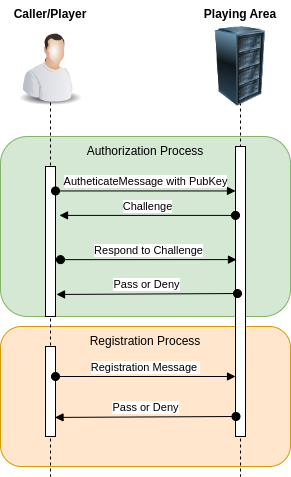
\includegraphics{AuthenticateUML.png}
\end{center}

\subsection{Deck and Card Generation}
Once the game automatically starts, the first step is to generate the deck using the procedure described in the project guidelines.\\
The \emph{playing area} notifies the \emph{caller} that the game has started and that they should generate the deck. The caller, that by now already knows how long the deck should be, generates a shuffled list of \textbf{N} numbers from 0 to \textbf{N-1} (where N is the deck size). Each element from this list is encrypted using their \emph{AES symmetric key} (known as deck key) and signed with their private playing key. \\
From here on out, this deck gets passed around to all players in sequential order. Each player encrypts the deck with their own deck key, shuffles it around and appends their signature to it. Once every user has done it, the deck goes back to the caller who signs it once more. \\
Now that the final version of the deck has been created, it is committed to the playing area for all to see. The players and caller must now make their deck key known so that they can reverse the process done to arrive at the original deck and every player’s card. \\
So now every user is decrypting and unshuffling the card in reverse order, verifying the signatures along the way. At the very end, they all will arrive at the unencrypted, original deck issued by the caller. If something goes wrong along the way, the game is aborted as someone is trying to cheat. \\
It’s important to note that every shuffling described in this section was done deterministically, using the deck key of the shuffler as seed, which was at that point a secret. Once they are known by all, the shuffling can be undone.\\
With the unencrypted deck known by all, each user can redo the shuffling in order to arrive at the unencrypted deck as shuffled by each player. The first \textbf{M} numbers are taken to be that player’s card, where \textbf{M} is the size of the card as determined by the playing area.

\subsection{Winner Detection}
At this point, every player and caller knows the original deck and each others cards in a way and knows that nobody could have cheated. \\
All that is left to do is to go through each card and see which one gets filled the earliest. There is always at least one winner. \\
The users don’t need to compare their findings as the process itself demands that no foul play must have taken place. Now that everyone knows who the winners are, they all cleanly disconnects from the playing area.
\begin{center}
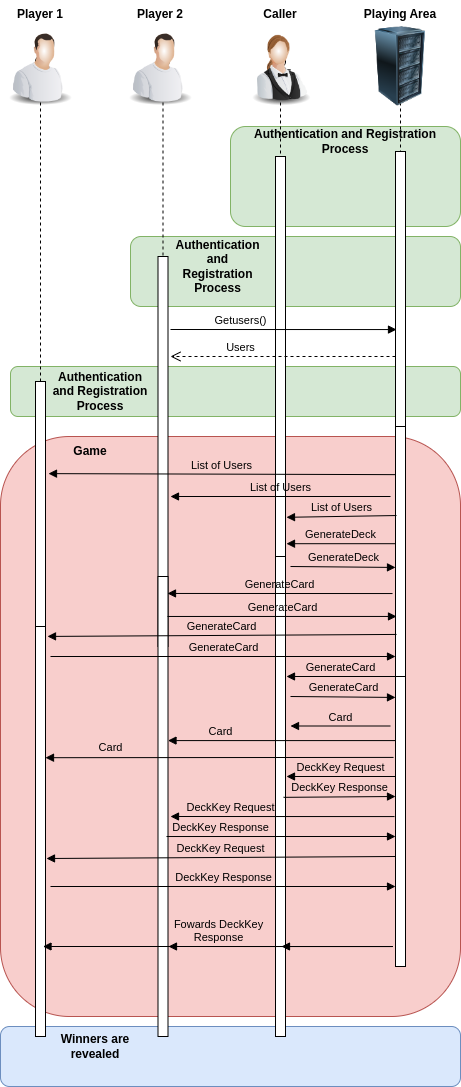
\includegraphics[scale=0.6]{flowchart.png}
\end{center}


\section{Changes From First Delivery}\label{changes}
\subsection{Smart Card Authentication}\label{smart card authentication}
Our first delivery did not include authentication using the Portuguese citizen smart card due to technical issues. We have added it in now.\\
We’ve created a new class “SmartCardSession” for handling PKCS11 sessions. It can sign data using the private key and share it’s public key in the form of a modulus and public exponent. We sign data using the SHA-256 hashing algorithm instead of SHA-1 (which was used in the practical classes) for increased robustness.\\
We used the PyKCS11 python module as a PKCS11 wrapper. It does not include a PKCS11 library, however, so we used OpenSC’s to that end.\\ 
\\
Signatures for SmartCardSession's methods in the smartcard\_reader.py.\\ 
Furthermore, we expanded the “crypto.py” cryptographic utility class to include methods for recreating  the RSA key object from the modulus and exponent as well as a method for verifying a digital signature from the smart card.

\begin{lstlisting}[captionpos=b label=listing:sparql_getallindividuals,
   basicstyle=\ttfamily]
import PyKCS11

# PyKCS11 does not include a PKCS11 library. We'll use opensc
#lib = '/usr/lib/x86_64-linux-gnu/pkcs11/opensc-pkcs11.so' # Mint location using apt install opensc-pkcs11
lib = '/usr/lib64/pkcs11/opensc-pkcs11.so' # Fedora location using dnf install opensc

class SmartCardSession():
    """Smart Card Session Utilities"""

    # static method for creating session object
    @classmethod
    def create(cls, pin : str) -> None:
        """Generates a PyKCS11 session, required Citizen Card PIN code"""
		...
		
    def getPublicKey(self) -> tuple[bytes, bytes]:
        """Returns the modulus and pubExponent corresponding to the smart card's public key as bytes"""
        ...

    def sign(self,message: bytes) -> bytes:
        """Signs a message and returns the signature"""
		...

    def close(self) -> None:
        """Closes the PyKCS11 session"""
        ...
        
\end{lstlisting}

The only other difference is that “Player.py” and “Caller.py” need an additional PIN parameter from creating the smart card session.

\subsection{AES Block Cipher Mode}\label{aes block Cipher Mode}
When faced with the choice of what block cipher mode of operation we should use with AES for symmetric encryption, we originally chose Galois Counter Mode (GCM).\\
Our reasoning for GCM to be the better choice was that it offered more features than the other modes, such as automatic integrity checking, higher tampering resistance, capability for pre-processing and parallel processing.\\
This conclusion proved to be foolhardy, as GCM was completely overkill for the use case of deck encryption, as pointed out by Professor Zúquete. It also added unnecessary complexity in the form of the IVs required for cipher operations.\\
As it turns out, the simpler Electronic Code Book (ECB) is a much better fit to our problem. It doesn’t boast as many qualities as GCM, but it’s good enough for our use case and doesn’t have unnecessary overhead for features we won’t use. Since decks don’t have repeating numbers, pattern propagation is not an issue either.\\
We learned a valuable lesson about the importance of carefully considering the requirements and constraints of a system to determine what technological solution best satisfies those needs, as opposed to instinctively going for the theoretically “best” option. Although GCM was supposedly the better choice, it’s advantages over ECB were superfluous to the needs of the system while keeping the complexity associated with them.
\\
\\
\begin{Large}
Previously, with GCM. Note that the same IV is used for every message, compromising robustness.
\end{Large} 
\begin{lstlisting}[captionpos=b label=listing:sparql_getallindividuals,
   basicstyle=\ttfamily]def sym_decrypt(cls, key: bytes, crypted_data, nonce: bytes=b'12345678') -> bytes:
        """Decrypts encrypted data given with given AESGCM key"""

        crypted_data=base64.b64decode(crypted_data.encode('ascii'))
        key=base64.b64decode(key.encode('ascii'))
        cypher = AESGCM(key) 
        data = cypher.decrypt(nonce, crypted_data, None)
         
        return data.decode('ascii')
\end{lstlisting}
\begin{Large}
Currently, with ECB.
\end{Large}
\begin{lstlisting}[captionpos=b label=listing:sparql_getallindividuals,
   basicstyle=\ttfamily]
def sym_encrypt(cls, key: bytes, data) -> bytes:
        """Encrypts data given with given AESGCM key"""
 
        key=base64.b64decode(key.encode('ascii'))
        data=bytes(str(data), 'ascii')

        cipher = Cipher(algorithms.AES(key), modes.ECB()) 

        # Set up padder
        padder = sym_padding.PKCS7(128).padder()
        
        # Add padding to the bites
        padded_data = padder.update(data) + padder.finalize() 

        # create encryptor
        encryptor = cipher.encryptor()

        # encrypt the message
        ct = encryptor.update(padded_data) + encryptor.finalize()

        return base64.b64encode(ct).decode('ascii')

\end{lstlisting}


\subsection{Cross Language Interoperability}\label{cross language interoperability}

Our system features a novel method for card generation, in which every player shuffles the playing deck as they sign it with their symmetric key.\\
Once the generation process has been completed and everyone knows the clear deck, users unshuffle the deck in the reverse order it was shuffled in to determine the card of every player. The first N numbers of the deck as shuffled by a given player is their playing card, where N is the card length.\\
More information about our method can be found at our previous report.\\
It was vital that whenever a user shuffles the deck, it is done deterministically as to allow the others users to unshuffle it. To achieve that, we used a method that deterministically shuffles and unshuffles a list given a seed. The seed is the player’s deck encryption key, as it is a secret up until the point everyone shares theirs at the end of the deck generation.\\
\begin{Large}
Original shuffling methods. Note the use of the random module.
\end{Large}
\begin{lstlisting}[captionpos=b label=listing:sparql_getallindividuals,
   basicstyle=\ttfamily]
    # https://crypto.stackexchange.com/q/78309
    def deterministic_shuffle(self, ls, seed : str):
        """Deterministically shuffles a list given a seed""" 
        random.seed(seed)
        random.shuffle(ls)
        return ls
    # https://crypto.stackexchange.com/q/78309
    def deterministic_unshuffle(self, shuffled_ls, seed : str):
        n = len(shuffled_ls)
        # perm is [1, 2, ..., n]
        perm = [i for i in range(1, n + 1)]
        # apply sigma to perm
        shuffled_perm = self.deterministic_shuffle(perm, seed)
        # zip and unshuffle
        zipped_ls = list(zip(shuffled_ls, shuffled_perm))
        zipped_ls.sort(key=lambda x: x[1])
        return [a for (a, b) in zipped_ls]
\end{lstlisting}
One issue we had not considered raised by Professor Zúquete is that our methods rely on Python’s module for random number generation. This means that a bingo client written in a programming language other than Python could not play with our Python client as it would shuffle the deck differently, even though they both follow the same communication protocol.\\
To fix this, we refactored those functions to use a cross-language method for random number generation. The solution we came up with is to hash the seed using MD5 and treating each of the sixteen bytes of the digest as a pool of random integers to be used by the Fisher-Yates list shuffling algorithm. If we run out of numbers in the pool, we generate it again using a different nonce.\\
\begin{Large}
Shuffling using MD5. The unshuffling method remains unaltered.
\end{Large}
\begin{lstlisting}[captionpos=b label=listing:sparql_getallindividuals,
   basicstyle=\ttfamily]
 # Fisher-Yates Algorithm https://favtutor.com/blogs/shuffle-list-python
    @classmethod
    def deterministic_shuffle(cls, ls : list, seed : str):
        """Deterministically shuffles a list given a seed using the Fisher-Yates Algorithm""" 

        rng = [] # array of 16 random numbers as generated from a MD5 hash
        nonce = 0 # nonce for generating the hash in case the original rng pool runs out
        for i in range(len(ls)-1, 0, -1):

            # if the random number pool is empty, generate more numbers 
            if rng == []:
                digest = hashlib.md5((seed+str(nonce)).encode()).digest() # MD5 hash of the seed + the nonce as a source of uniqueness
                rng = [x for x in digest] # convert bytes to array of ints
                nonce += 1 # increase the nonce so that the next digest is different

            # selects a random index using the random number
            j = rng.pop() % i
            ls[i],ls[j] = ls[j], ls[i] # swaps two items
        
        return ls

    # https://crypto.stackexchange.com/q/78309
    @classmethod
    def deterministic_unshuffle(cls, shuffled_ls : list, seed : str):
        """Reverses the deterministic shuffle and returns the original list"""
        n = len(shuffled_ls)
        # perm is [1, 2, ..., n]
        perm = [i for i in range(1, n + 1)]
        # apply sigma to perm
        shuffled_perm = cls.deterministic_shuffle(perm, seed)
        # zip and unshuffle
        zipped_ls = list(zip(shuffled_ls, shuffled_perm))
        zipped_ls.sort(key=lambda x: x[1])
        return [a for (a, b) in zipped_ls]
\end{lstlisting}

\section{Protocol}\label{protocol}


Communication Protocol and Cryptography Protocol documentation.

\subsection{Communication Protocol}\label{communication-protocol}

\subsubsection{Messages}\label{messages}

\begin{itemize}
\item
  \textbf{Message} 
  \begin{longtable}[]{@{}ll@{}}
  \toprule
  \endhead
  \begin{minipage}[t]{0.40\columnwidth}\raggedright
  Description\strut
  \end{minipage} & \begin{minipage}[t]{0.54\columnwidth}\raggedright
  Generic message\strut
  \end{minipage}\tabularnewline
  \begin{minipage}[t]{0.40\columnwidth}\raggedright
  Methods\strut
  \end{minipage} & \begin{minipage}[t]{0.54\columnwidth}\raggedright
  \begin{itemize}
  	\item to\_json()
  	\item should\_log()
  \end{itemize}\strut
  \end{minipage}\tabularnewline
  \bottomrule
  \end{longtable}

\item

  \textbf{Authorization} 
  \begin{longtable}[]{@{}ll@{}}
  \toprule
  \endhead
  \begin{minipage}[t]{0.40\columnwidth}\raggedright
  Description\strut
  \end{minipage} & \begin{minipage}[t]{0.54\columnwidth}\raggedright
  Message for Users to authenticate themselves to the playing area. Uses
  challenge-response authenticatio\strut
  \end{minipage}\tabularnewline
  \begin{minipage}[t]{0.40\columnwidth}\raggedright
  Extends\strut
  \end{minipage} & \begin{minipage}[t]{0.54\columnwidth}\raggedright
  Message\strut
  \end{minipage}\tabularnewline
  \begin{minipage}[t]{0.40\columnwidth}\raggedright
  Methods\strut
  \end{minipage} & \begin{minipage}[t]{0.54\columnwidth}\raggedright
  \begin{itemize}
  	\item parse()
  \end{itemize}\strut
  \end{minipage}\tabularnewline
  \bottomrule
  \end{longtable}
\item
  \textbf{Register}

  \begin{longtable}[]{@{}ll@{}}
  \toprule
  \endhead
  \begin{minipage}[t]{0.40\columnwidth}\raggedright
  Description\strut
  \end{minipage} & \begin{minipage}[t]{0.54\columnwidth}\raggedright
  Message for players to register themselves to the playing area\strut
  \end{minipage}\tabularnewline
  \begin{minipage}[t]{0.40\columnwidth}\raggedright
  Extends\strut
  \end{minipage} & \begin{minipage}[t]{0.54\columnwidth}\raggedright
  Message\strut
  \end{minipage}\tabularnewline
  \begin{minipage}[t]{0.40\columnwidth}\raggedright
  Methods\strut
  \end{minipage} & \begin{minipage}[t]{0.54\columnwidth}\raggedright
  parse()\strut
  \end{minipage}\tabularnewline
  \begin{minipage}[t]{0.40\columnwidth}\raggedright
  Parameters\strut
  \end{minipage} & \begin{minipage}[t]{0.54\columnwidth}\raggedright
  \begin{itemize}
  	\item nickname
  	\item   playing\_key
  	\item   auth\_key
	\item signature
	\item success
	\item sequence
  \end{itemize}\strut
  \end{minipage}\tabularnewline
  \bottomrule
  \end{longtable}

\item
  \textbf{GetUsers}

  \begin{longtable}[]{@{}ll@{}}
  \toprule
  \endhead
  Description & Message for getting a list of registered
  users\tabularnewline
  Extends & Message\tabularnewline
  Methods & parse(), should\_log() \textbf{returns false}\tabularnewline
  \begin{minipage}[t]{0.40\columnwidth}\raggedright
  Parameters\strut
  \end{minipage} & \begin{minipage}[t]{0.54\columnwidth}\raggedright
  \begin{itemize}
  	\item public\_key
	\item signature
	\item response
  \end{itemize}\strut
  \end{minipage}\tabularnewline
  \bottomrule
  \end{longtable}

\item
  \textbf{CardSize}

  
  \begin{longtable}[]{@{}ll@{}}
  \toprule
  \endhead
  Description & Simple message for letting users know the card size \tabularnewline
  Extends & Message\tabularnewline
  Methods & parse(), should\_log() \textbf{returns false}\tabularnewline
  \begin{minipage}[t]{0.40\columnwidth}\raggedright
  Parameters\strut
  \end{minipage} & \begin{minipage}[t]{0.54\columnwidth}\raggedright
  \begin{itemize}
  	\item card\_size
  \end{itemize}\strut
  \end{minipage}\tabularnewline
  \bottomrule
  \end{longtable}
\item
  \textbf{GetLog}


  \begin{longtable}[]{@{}ll@{}}
  \toprule
  \endhead
  Description & Message for getting a list of logged messages \tabularnewline
  Extends & Message\tabularnewline
  Methods & parse(), should\_log() \textbf{returns false}\tabularnewline
  \begin{minipage}[t]{0.40\columnwidth}\raggedright
  Parameters\strut
  \end{minipage} & \begin{minipage}[t]{0.54\columnwidth}\raggedright
  \begin{itemize}
  	\item public\_key
  	\item signature
  	\item response
  \end{itemize}\strut
  \end{minipage}\tabularnewline
  \bottomrule
  \end{longtable}

\item
  \textbf{PartyUpdate}

  \begin{longtable}[]{@{}ll@{}}
  \toprule
  \endhead
  Description & Message for updating registered users on how big the party is \tabularnewline
  Extends & Message\tabularnewline
  Methods & parse(), should\_log() \textbf{returns false}\tabularnewline
  \begin{minipage}[t]{0.40\columnwidth}\raggedright
  Parameters\strut
  \end{minipage} & \begin{minipage}[t]{0.54\columnwidth}\raggedright
  \begin{itemize}
  	\item signature
  	\item public\_key
  	\item response
  \end{itemize}\strut
  \end{minipage}\tabularnewline
  \bottomrule
  \end{longtable}

\item
  \textbf{GenerateDeck} 

	
  \begin{longtable}[]{@{}ll@{}}
  \toprule
  \endhead
  \begin{minipage}[t]{0.40\columnwidth}\raggedright
  Description\strut
  \end{minipage} & \begin{minipage}[t]{0.54\columnwidth}\raggedright
   Message telling the caller to generate the deck and initiate the card generation proccess\strut
  \end{minipage}\tabularnewline
  Extends & Message\tabularnewline
  Methods & parse()\tabularnewline
  \begin{minipage}[t]{0.40\columnwidth}\raggedright
  Parameters\strut
  \end{minipage} & \begin{minipage}[t]{0.54\columnwidth}\raggedright
  \begin{itemize}
  	\item deck\_size
  \end{itemize}\strut
  \end{minipage}\tabularnewline
  \bottomrule
  \end{longtable}  
  
\item
  \textbf{GenerateCard}

  
  \begin{longtable}[]{@{}ll@{}}
  \toprule
  \endhead
  \begin{minipage}[t]{0.40\columnwidth}\raggedright
  Description\strut
  \end{minipage} & \begin{minipage}[t]{0.54\columnwidth}\raggedright
   Message Players will pass around until everyone has commited their card\strut
  \end{minipage}\tabularnewline
  Methods & parse(), sign(), verify\tabularnewline
  \begin{minipage}[t]{0.40\columnwidth}\raggedright
  Parameters\strut
  \end{minipage} & \begin{minipage}[t]{0.54\columnwidth}\raggedright
  \begin{itemize}
  	\item sequence (int)
  	\item deck (list)
	\item signatures (list)
	\item done (bool)
  \end{itemize}\strut
  \end{minipage}\tabularnewline
  \bottomrule
  \end{longtable}  

  Methods 
  \begin{itemize}
  
	\item sign(private\_key : str)

  \textbf{Description}: Signs the deck with private\_Key and append the
  public key to the signatures array Call our Cryptography function
  \textbf{sign}

  \item verify(publicKey : str, signature)

  \textbf{Description}: Verifies the signature of the deck with the
  public key Call our Cryptography function \textbf{verify}  
  
  \end{itemize}
 
\item
  \textbf{DeckKeyRequest}

  \begin{longtable}[]{@{}ll@{}}
  \toprule
  \endhead
  \begin{minipage}[t]{0.40\columnwidth}\raggedright
  Description\strut
  \end{minipage} & \begin{minipage}[t]{0.54\columnwidth}\raggedright
  Message requesting that players and caller reveal their symmetric key
  after the deck is commited\strut
  \end{minipage}\tabularnewline
  \begin{minipage}[t]{0.40\columnwidth}\raggedright
  Extends\strut
  \end{minipage} & \begin{minipage}[t]{0.54\columnwidth}\raggedright
  Message\strut
  \end{minipage}\tabularnewline
  \begin{minipage}[t]{0.40\columnwidth}\raggedright
  Methods\strut
  \end{minipage} & \begin{minipage}[t]{0.54\columnwidth}\raggedright
  parse()\strut
  \end{minipage}\tabularnewline
  \begin{minipage}[t]{0.40\columnwidth}\raggedright
  Parameters\strut
  \end{minipage} & \begin{minipage}[t]{0.54\columnwidth}\raggedright
  sequence\strut
  \end{minipage}\tabularnewline
  \bottomrule
  \end{longtable}


\item
  \textbf{DeckKeyResponse}

	
  \begin{longtable}[]{@{}ll@{}}
  \toprule
  \endhead
  \begin{minipage}[t]{0.40\columnwidth}\raggedright
  Description\strut
  \end{minipage} & \begin{minipage}[t]{0.54\columnwidth}\raggedright
  Response to the deck key request \strut
  \end{minipage}\tabularnewline
  \begin{minipage}[t]{0.40\columnwidth}\raggedright
  Extends\strut
  \end{minipage} & \begin{minipage}[t]{0.54\columnwidth}\raggedright
  Message\strut
  \end{minipage}\tabularnewline
  \begin{minipage}[t]{0.40\columnwidth}\raggedright
  Methods\strut
  \end{minipage} & \begin{minipage}[t]{0.54\columnwidth}\raggedright
  parse(), sign()\strut
  \end{minipage}\tabularnewline
  \begin{minipage}[t]{0.40\columnwidth}\raggedright
  Parameters\strut
  \end{minipage} & \begin{minipage}[t]{0.54\columnwidth}\raggedright
  \begin{itemize}
  	\item sequence
  	\item response
  	\item signature
  \end{itemize}
  \end{minipage}\tabularnewline
  \bottomrule
  \end{longtable}
	
\item
  \textbf{GameOver}

  \begin{longtable}[]{@{}ll@{}}
  \toprule
  \endhead
  Description & Message for when the game is over /
  aborted\tabularnewline
  Extends & Message\tabularnewline
  Methods & parse() should\_log() \textbf{returns false} \_\_ str
  \_\_()\tabularnewline
  \begin{minipage}[t]{0.40\columnwidth}\raggedright
  Parameters\strut
  \end{minipage} & \begin{minipage}[t]{0.54\columnwidth}\raggedright
  \begin{itemize}
  	\item status
  \end{itemize}\strut
  \end{minipage}\tabularnewline
  \bottomrule
  \end{longtable}

\end{itemize}

\subsection{Cryptography Protocol, Crypto
(Class)}\label{cryptography-protocol-crypto-class}

Cryptographic utilities

Uses \textbf{cryptography.hazmat.primitives}

\subsubsection{Methods}\label{methods}

\begin{itemize}
\item
  \textbf{sym\_gen} 
	
	
  \begin{longtable}[]{@{}ll@{}}
  \toprule
  \endhead
  Description & Generates a new AESGCM (key, nonce) tuple\tabularnewline
  \begin{minipage}[t]{0.40\columnwidth}\raggedright
  Parameters\strut
  \end{minipage} & \begin{minipage}[t]{0.54\columnwidth}\raggedright
\strut
  \end{minipage}\tabularnewline
  \begin{minipage}[t]{0.40\columnwidth}\raggedright
  Return\strut
  \end{minipage} & \begin{minipage}[t]{0.54\columnwidth}\raggedright
	tuple \strut
  \end{minipage}\tabularnewline
  \bottomrule
  \end{longtable}
  
  
\item
  \textbf{sym\_encrypt} 
  
		
  \begin{longtable}[]{@{}ll@{}}
  \toprule
  \endhead
  Description & Encrypts data given with given AESGCM key\tabularnewline
  \begin{minipage}[t]{0.40\columnwidth}\raggedright
  Parameters\strut
  \end{minipage} & \begin{minipage}[t]{0.54\columnwidth}\raggedright
  \begin{itemize}
  	\item key: bytes
  	\item data
  	\item  nonce: bytes
  \end{itemize} \strut
  \end{minipage}\tabularnewline
  \begin{minipage}[t]{0.40\columnwidth}\raggedright
  Return \strut
  \end{minipage} & \begin{minipage}[t]{0.54\columnwidth}\raggedright
	bytes \strut
  \end{minipage}\tabularnewline
  \bottomrule
  \end{longtable}
  
  


\item
  \textbf{sym\_decrypt} 
  
  	
  \begin{longtable}[]{@{}ll@{}}
  \toprule
  \endhead
  Description & Decrypts encrypted data given with given AESGCM key\tabularnewline
  \begin{minipage}[t]{0.40\columnwidth}\raggedright
  Parameters\strut
  \end{minipage} & \begin{minipage}[t]{0.54\columnwidth}\raggedright
  \begin{itemize}
  	\item key: bytes
  	\item crypted\_data
  	\item  nonce: bytes
  \end{itemize} \strut
  \end{minipage}\tabularnewline
  \begin{minipage}[t]{0.40\columnwidth}\raggedright
  Return \strut
  \end{minipage} & \begin{minipage}[t]{0.54\columnwidth}\raggedright
	bytes \strut
  \end{minipage}\tabularnewline
  \bottomrule
  \end{longtable}
  
\item
  \textbf{do\_hash}

  \begin{longtable}[]{@{}ll@{}}
  \toprule
  \endhead
  Description & Returns an hash of a given data; Uses
  SHA256\tabularnewline
  Parameters & data: bytes\tabularnewline
  Return & bytes\tabularnewline
  \bottomrule
  \end{longtable}
\item
  \textbf{asym\_gen}

  \begin{longtable}[]{@{}ll@{}}
  \toprule
  \endhead
  Description & Encrypts data using given public key\tabularnewline
  Parameters &\tabularnewline
  Return & bytes\tabularnewline
  \bottomrule
  \end{longtable}
  
\item
  \textbf{sign}
  \begin{longtable}[]{@{}ll@{}}
  \toprule
  \endhead
   \begin{minipage}[t]{0.40\columnwidth}\raggedright
  Description\strut
  \end{minipage} & \begin{minipage}[t]{0.54\columnwidth}\raggedright
    Returns Signature of given data signed with given private key; Uses SHA256
\strut
  \end{minipage}\ 
  \tabularnewline
  \begin{minipage}[t]{0.40\columnwidth}\raggedright
  Parameters\strut
  \end{minipage} & \begin{minipage}[t]{0.54\columnwidth}\raggedright
  \begin{itemize}
  	\item private\_key
  	\item data
  \end{itemize} \strut
  \end{minipage}\tabularnewline
  \begin{minipage}[t]{0.40\columnwidth}\raggedright
  Return \strut
  \end{minipage} & \begin{minipage}[t]{0.54\columnwidth}\raggedright
	bytes \strut
  \end{minipage}\tabularnewline
  \bottomrule
  \end{longtable}
  
\item
  \textbf{verify}


  \begin{longtable}[]{@{}ll@{}}
  \toprule
  \endhead
   \begin{minipage}[t]{0.40\columnwidth}\raggedright
  Description\strut
  \end{minipage} & \begin{minipage}[t]{0.54\columnwidth}\raggedright
    Verifies if given message matches with given signature; Uses SHA256
  \strut
  \end{minipage}\ 
  \tabularnewline
  \begin{minipage}[t]{0.40\columnwidth}\raggedright
  Parameters\strut
  \end{minipage} & \begin{minipage}[t]{0.54\columnwidth}\raggedright
  \begin{itemize}
  	\item public\_key
  	\item signature: bytes
  	\item message
  \end{itemize} \strut
  \end{minipage}\tabularnewline
  \begin{minipage}[t]{0.40\columnwidth}\raggedright
  Return \strut
  \end{minipage} & \begin{minipage}[t]{0.54\columnwidth}\raggedright
	bool \strut
  \end{minipage}\tabularnewline
  \bottomrule
  \end{longtable}
  


  

\end{itemize}

\end{document}
